%-------------------------------------------------------------------------------
%-------------------------------------------------------------------------------
%-------------------------------------------------------------------------------
\chapter{Équations différentielles : compléments}
%-------------------------------------------------------------------------------
%-------------------------------------------------------------------------------
\thispagestyle{empty}
%-------------------------------------------------------------------------------
%-------------------------------------------------------------------------------
%-------------------------------------------------------------------------------
{\sf Ce chapitre présente des développements du chapitre sur les équations différentielles qu'une lecture raisonnable du programme peut considérer comme hors-programme mais que les épreuves des concours et les calculs en T.I.P.E. utilisent couramment.

Le texte utilise la fonction \type{Euler} de résolution mais on peut lui substituer toute autre méthode vue dans le T.P. Il est en fait recommander d'utiliser la fonction \type{odeint} du module \type{scipy.integrate} qui se substitue efficacement aux fonctions écrites.}
%-------------------------------------------------------------------------------
%-------------------------------------------------------------------------------
%-------------------------------------------------------------------------------
\section{Équations d'ordre 2}
%-------------------------------------------------------------------------------
%-------------------------------------------------------------------------------
%-------------------------------------------------------------------------------
\subsection{Exemple}
%-------------------------------------------------------------------------------
%-------------------------------------------------------------------------------
\begin{minipage}{.65\linewidth}
Le pendule pesant est soumis à la force de la pesanteur et à la réaction du fil ($\overrightarrow{R}$). La formule de Newton donne, en projetant dans une base orthonormée directe $(\overrightarrow{u_r}, \overrightarrow{u_\theta})$ telle que $\overrightarrow{OM} = l\overrightarrow{u_r}$,
\begin{align}
 -ml\left(\frac {d \theta}{d t}\right)^2 = -R + mg\cos(\theta)\hfill\\
  ml\frac {d^2 \theta}{d t^2} = -mg\sin(\theta)\qquad
 \end{align}
On remarque que la la seconde équation, obtenue en projetant sur $\overrightarrow{u_\theta}$ ne fait intervenir que l'angle comme fonction du temps mais elle fait intervenir la dérivée seconde.

La première équation, obtenue en projetant sur $\overrightarrow{u_r}$, permet de calculer $R(t)$ si on connaît la fonction $\theta(t)$.
\end{minipage} 
\hskip 5mm
%--------------------------------------------------------------------------
\begin{minipage}[c]{.30\linewidth}
\begin{center}
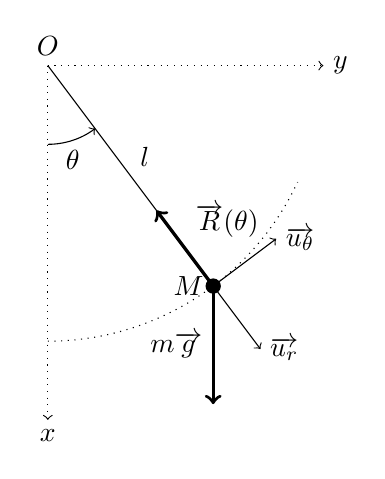
\begin{tikzpicture}
\draw (0,0) node[above] {$O$} -- node[above right] {$l$} (2.1, -2.8) node [left] {$M$};
\draw[dotted,->] (0,0) -- (0, -4.5) node [below]{$x$};
\draw[dotted,->] (0,0) -- (3.5, 0) node [right]{$y$};
\draw[fill] (2.1, -2.8) circle (0.09);
\draw[->] (0, -1) arc (-90:-53:1) node [midway, below] {$\theta$};
\draw[dotted] (0, -3.5) arc (-90:-25:3.5) ;
\draw[very thick, ->] (2.1, -2.8) -- node [left] {$m\overrightarrow g$} +(0, -1.5);
\draw[very thick, ->] (2.1, -2.8) -- node [above right] {$\overrightarrow R(\theta)$} +(-0.72, 0.96);
\draw[->] (2.1, -2.8) -- +(0.6, -0.8) node [right] {$\overrightarrow{u_r}$};
\draw[->] (2.1, -2.8) -- +(0.8,  0.6) node [right] {$\overrightarrow{u_\theta}$};
%\draw[->] (2.1, -2.8) -- node [above right] {$\vec a$} +(-0.72, -0.54);
\end{tikzpicture}  
\end{center}
\end{minipage}  
%-------------------------------------------------------------------------------
\newpage
%-------------------------------------------------------------------------------
\subsection{Un solution} \label{sec:sol}
%-------------------------------------------------------------------------------
%-------------------------------------------------------------------------------
Une équation différentielle d'ordre 2 est une équation qui exprime la dérivée seconde en fonction des valeurs de la fonction, de sa dérivée et de la variable.
\[y'' = \psi(y, y', t)\]
Dans l'exemple ci-dessus $\psi(y, y', t) = -\frac g l \sin(y)$.

\medskip

Une propriété importante des équation différentielle d'ordre 2 est qu'une des conditions pour qu'existe une solution unique est qu'on doit donner des conditions initiales en $t_0$ pour la fonction et pour sa dérivée\footnote{Le cas des conditions aux limites, $y(t_0) = y_0$ et $y(t_{final}) = y_{final}$, plus difficile, ne sera pas traité ici.}.

On peut alors résoudre de manière approchée l'équation avec des approximations d'Euler à 2 étages : on incluant le calcul des dérivées aux temps $t_i$. 

On cherchera donc à définir deux listes \type{Y}, pour les valeurs de la fonctions, et \type{V}, pour les valeurs de sa dérivée. La valeur de \type{Y[i]}, $y_i$, et celle de \type{V[i]}, $v_i$ seront des valeurs approchées de $f(t_i)$ et $f'(t_i)$ respectivement où $f$ est la solution telle que $f(t_0) = y_0$ et $f'(t_0)= v_0$.

Si on note $h_i = t_{i+1} - t_i$, on calcule donc itérativement 
\[y_{i+1}\simeq f(t_{i+1}) \simeq f(t_i) + \delta_i f'(t_i)  \simeq y_i + h_i v_i\hbox{ et }\]
\[v_{i+1}\simeq f'(t_{i+1}) \simeq f'(t_i) + h_if''(t_i) = f'(t_i) + h_i\psi\bigl(f(t_i), f'(t_i),  t_i\bigr)\simeq v_i + h_i\psi(y_i, v_i, t_i)\]
%-------------------------------------------------------------------------------
\begin{lstlisting}
def Euler2(psi, y0, v0, T):
    n = len(T)           
    Y = [0]*n 
    Y[0] = y0 
    V = [0]*n 
    V[0] = v0 
    for i in range(n-1): 
        pas = T[i+1] - T[i]
        Y[i+1] = Y[i] + pas*V[i]
        V[i+1] = V[i] + pas*psi(Y[i], V[i], T[i])
    return Y, V
\end{lstlisting}
%-------------------------------------------------------------------------------
Les deux listes \type{Y} et \type{V} permettent de tracer le {\bf portrait de phase} où, au lieu de représenter $y$ en fonction de $t$, on représente la trajectoire des points de coordonnées $\bigl(y(t), y'(t)\bigr)$.
%-------------------------------------------------------------------------------
%-------------------------------------------------------------------------------
\subsection{Traitement de l'exemple}
%-------------------------------------------------------------------------------
%-------------------------------------------------------------------------------
On revient à l'exemple $\theta''(t) = -\frac g l \sin\bigl(\theta(t)\bigr)$.
%-------------------------------------------------------------------------------
\begin{lstlisting}
import numpy as np
import matplotlib.pyplot as plt

g = 9.81
l = 0.5 
t_fin = 10 # temps final pour l'étude
N  = 100000  # nombre de points
T = np.linspace(0, t_fin, N)

def psi(y, v, t):
    return -g/l*np.sin(y)
\end{lstlisting}
%-------------------------------------------------------------------------------
\newpage
%-------------------------------------------------------------------------------
%-------------------------------------------------------------------------------
\begin{itemize}
    \item On peut tracer une solution et la courbe des vitesses, par exemple pour $\theta_0 = \frac \pi 6$ et $v_0=0$.
%-------------------------------------------------------------------------------
\begin{lstlisting}
y0 = np.pi/6
v0 = 0
Y, V = Euler2(psi, y0, v0, T)

plt.plot(T, Y, label = "Angle")
plt.plot(T, V, linestyle = "dashed", label = "Vitesse")
plt.legend()
plt.show()
\end{lstlisting}
%-------------------------------------------------------------------------------
\begin{center}
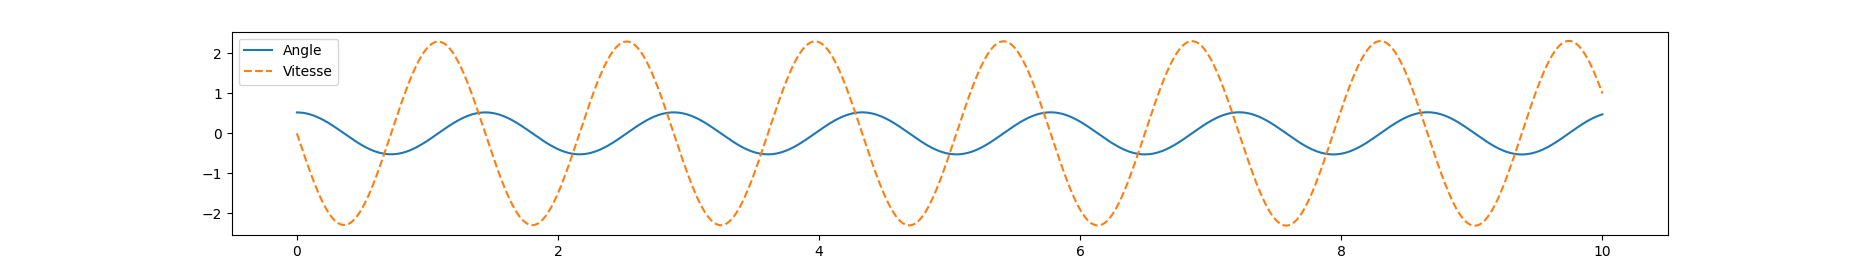
\includegraphics[width=14cm]{Cours/Images/ED2_pendule1.png}
\end{center}
%-------------------------------------------------------------------------------
\item On peut tracer plusieurs solution, on remarque que, contrairement à l'oscillateur harmonique, la période n'est pas constante.
%-------------------------------------------------------------------------------
\begin{lstlisting}
Y0 = [0.3, 0.6, 0.9, 1.2, 1.5]
v0 = 0
for y0 in Y0:
    Y, V = Euler2(psi, y0, v0, T)
    plt.plot(T, Y)
plt.show()
\end{lstlisting}
%-------------------------------------------------------------------------------
\begin{center}
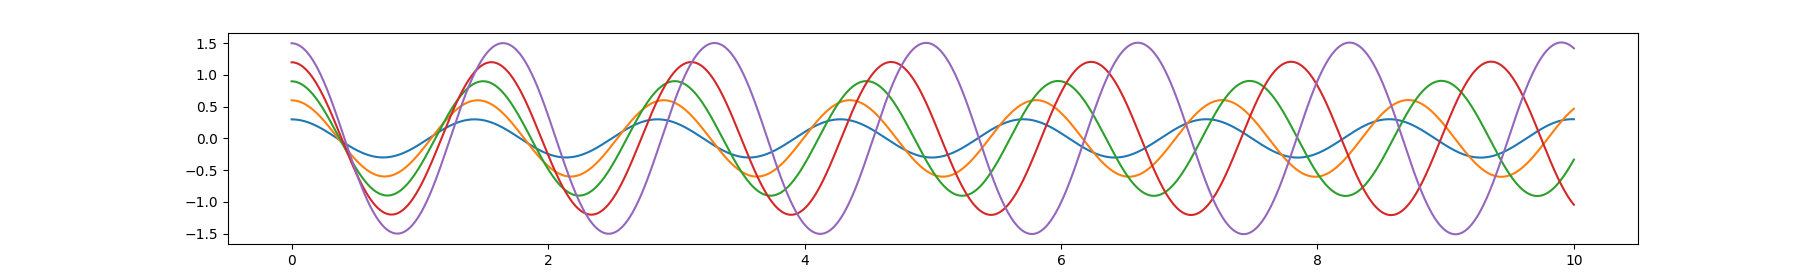
\includegraphics[width=14cm]{Cours/Images/ED2_pendule2.png}
\end{center}
%-------------------------------------------------------------------------------
\item On peut tracer plusieurs portraits de phases.
%-------------------------------------------------------------------------------
\begin{lstlisting}
Y0 = [0.5, 1.0, 1.5, 2.0, 2.5]
v0 = 0
for y0 in Y0:
    Y, V = Euler2(psi, y0, v0, T)
    plt.plot(Y, V)
plt.show()
\end{lstlisting}
%-------------------------------------------------------------------------------
\begin{center}
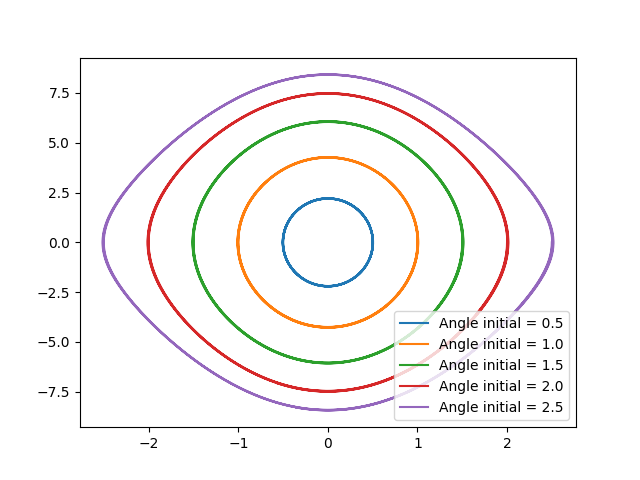
\includegraphics[width=8cm]{Cours/Images/ED2_pendule3.png}
\end{center}
\end{itemize}
%-------------------------------------------------------------------------------
%-------------------------------------------------------------------------------
%-------------------------------------------------------------------------------
\section{Équations couplées}
%-------------------------------------------------------------------------------
%-------------------------------------------------------------------------------
%-------------------------------------------------------------------------------
\subsection{Exemple}
%-------------------------------------------------------------------------------
%-------------------------------------------------------------------------------
\def\F{\text{F}}
\def\G{\text{G}}
\def\MV{\text{Mo(V)}}
\def\MVI{\text{Mo(VI)}}
\def\IV{\text{MoO}_{4}^{2-}}
\def\IVI{\text{MoO}_2^+}
Le fructose et le glucose sont deux sucres d'origine naturelle que l'on rencontre souvent en mélange. Leur dosage est important en particulier dans le sérum sanguin pour l'étude des maladies telles que le diabète. On propose ici d'étudier un dosage par une méthode cinétique fondée sur le fait que le glucose et le fructose réagissent à des vitesses différentes sur la plupart des réactifs. 

Le fructose noté F ainsi que le glucose G réduisent le molybdène (VI) présent sous la forme d'ions molybdate $\IV$ en ions $\IVI$ du molybdène (V) (bleu de molybdène) selon les réactions symbolisées :


%-------------------------------------------------------------------------------
\def\direct#1^#2_#3{%
\quad\mathrel{\mathop{\hbox to #1{\rightarrowfill}}\limits^{\textstyle #2}_{\textstyle #3}}\quad}
%-------------------------------------------------------------------------------
$$\begin{tabular}{rclcrcl}
Mo(VI) &+& F  &$\direct{2 cm}^{k_F}_{}$ & Mo(V) &+& $\F'$\\
Mo(VI) &+& G  &$\direct{2 cm}^{k_G}_{}$ & Mo(V) &+& $\G'$\\
\end{tabular}$$

Les composés sont des solutés et on note $[X]$ la concentration molaire volumique de $X$.

Les concentration initiales et à l'instant $t$ sont données par le tableau :
\[
\begin{tabular}{c|cccccc}
      & $[\MVI]$ & $[\F]$ & $[\G]$ & $[\MV]$ & $[\F']$ & $[\G']$\\[1mm]
\hline
$t=0$ &  $a$     & $b$    & $c$    &  0      &  0      & 0 \rule{0cm}{4mm}\\
$t$   & $a-x-y$  & $b-x$  & $c-y$ & $x+y$   & $x$     & $y$ \\
\end{tabular}
\]
La température et le volume sont maintenus constants, on suppose que les réactions sont d'ordre 1 par rapport à chacun des réactifs.

Les constantes de vitesses permettent de définir les relations
\[\left\{
\begin{matrix}
  \displaystyle \frac{\d [\F']}{\d t} = -\frac{\d [\F]}{\d t} = \frac{\d x}{\d t} = k_F[\MVI][\F] = k_F(a - x - y)(b-x)\\[3mm]
  \displaystyle \frac{\d [\G']}{\d t} = -\frac{\d [\G]}{\d t} = \frac{\d y}{\d t} = k_G[\MVI][\G] = k_G(a - x - y)(c-y)\\
\end{matrix}
\right.\]

Les valeurs numériques, exprimées en $\text{mol}\cdot \text{L}^{-1}$ pour les concentrations et en $\text{min}^{-1}\cdot \text{mol}^{-1}\cdot \text{L}$ pour les constantes de vitesse sont définies comme des variables globales.
%-------------------------------------------------------------------------------
\begin{lstlisting}
a  = 12.0e-2
b  =  3.0e-2
c  =  5.0e-2
kF =  7.8
kG  = 2.0
\end{lstlisting}
%-------------------------------------------------------------------------------
On voit que les deux équations différentielles ne peuvent pas être résolues indépendemment : elles sont {\bf couplées}, la dérivée de chacune des deux fonctions $x(t)$ et $y(t)$ dépend des deux fonctions.
%-------------------------------------------------------------------------------
%-------------------------------------------------------------------------------
\subsection{Une solution sans nouvelle fonction}
%-------------------------------------------------------------------------------
%-------------------------------------------------------------------------------
On pourrait, comme ci-dessus, utiliser la méthode d'Euler pour chaque équation en les résolvant en même temps : on devrait avoir pour paramètres les 2 équations et les deux conditions initiales. Pour les systèmes à 3, 4, \dots équations on devrait alors écrire une méthode de résolution différente.

Pour simplifier les choses on va utiliser la méthode de vectorisation : au lieu de considérer $n$ équations avec chacune une inconnue, on considère une seule équation avec $n$ inconnues. On fera plusieurs calculs en même temps en regroupant les différentes valeurs dans un {\bf vecteur}.

Dans l'exemple ci-dessus on considère donc le vecteur $u(t) = \begin{pmatrix} x(t)\\ y(t) \end{pmatrix}$.

En dérivant le vecteur terme-à-terme on obtient 
\[u'(t) 
= \begin{pmatrix} x'(t)\\ y'(t) \end{pmatrix}
= \begin{pmatrix}k_F\bigl(a - x(t) - y(t)\bigr)\bigl(b-x(t)\bigr)\\
k_G\bigl(a - x(t) - y(t)\bigr)\bigl(c-y(t)\bigr)\end{pmatrix}
= \Phi\bigl(u(t), t\bigr)
\]
Comme d'habitude on considère que la variable $t$ peut intervenir dans la dérivée.

\medskip
Les deux formules obtenues à partir de la méthode d'Euler :
\[\begin{matrix} x(t_{k+1}) \simeq x(t_k) + (t_{k+1}-t_k)x'(t_k)\\
y(t_{k+1}) \simeq y(t_k) + (t_{k+1}-t_k)y'(t_k)\end{matrix}
\]

deviennent $u(t_{k+1}) \simeq u(t_k) + (t_{k+1}-t_k)u'(t_k)=
u(t_k) + (t_{k+1}-t_k)\Phi\bigl(u(t_k), t_k\bigr)$.

On est revenu à un schéma d'Euler simple. Il faut simplement pouvoir multiplier les vecteurs par un scalaire et additionner 2 vecteurs, c'est que permettent directementles tableaux \type{numpy}.

Il reste donc à adapter est fonction de l'équation différentielle qui doit recevoir comme première variable un tableau \type{numpy} et renvoyer un tableau \type{numpy} de même taille. L'ensemble des conditions initiales devra aussi être défini par un tableau \type{numpy}.

On utilisera ensuite la fonction \type{Euler} (ou \type{odeint}) du chapitre précédent.
%-------------------------------------------------------------------------------
%-------------------------------------------------------------------------------
\subsection{Traitement de l'exemple}
%-------------------------------------------------------------------------------
%-------------------------------------------------------------------------------
On commence par la fonction : elle déconstruit le vecteur et en construit un nouveau.
%-------------------------------------------------------------------------------
\begin{lstlisting}
def phi(u, t):
    x, y = u
    dx = kF*(a - x - y)*(b - x)
    dy = kG*(a - x - y)*(c - y)
    return np.array([dx, dy])
\end{lstlisting}
%-------------------------------------------------------------------------------
Les conditions initiales sont regroupées dans un vecteur.
%-------------------------------------------------------------------------------
\begin{lstlisting}
T = np.linspace(0, 60, 10000)
u0 = np.array([0, 0])
U = Euler(phi, u0, T)
\end{lstlisting}
%-------------------------------------------------------------------------------
Le résultat est une liste de vecteurs, on va définir les listes de composantes.
%-------------------------------------------------------------------------------
\begin{lstlisting}
X = [u[0] for u in U]
Y = [u[1] for u in U]
plt.plot(T, X, label = "Fructose")
plt.plot(T, Y, label = "Glucose")
plt.legend()
plt.show()
\end{lstlisting}
%-------------------------------------------------------------------------------
%-------------------------------------------------------------------------------
\begin{center}
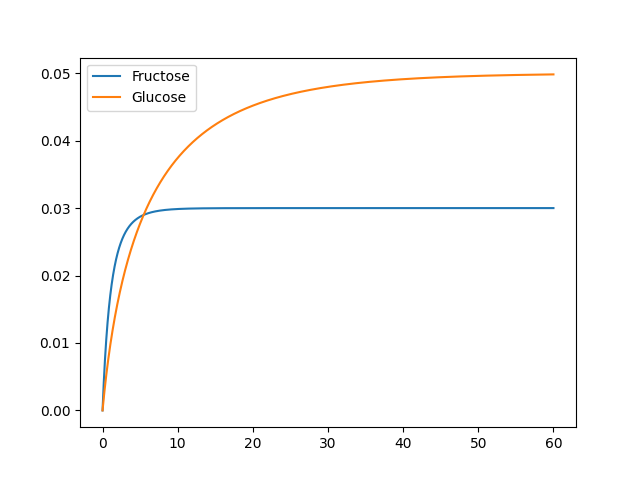
\includegraphics[width=8cm]{Cours/Images/ED2_glucose.png}
\end{center}
%-------------------------------------------------------------------------------
\newpage
%-------------------------------------------------------------------------------
%-------------------------------------------------------------------------------
\subsection{Retour sur les équations d'ordre 2}
%-------------------------------------------------------------------------------
%-------------------------------------------------------------------------------
La méthode vue dans le paragraphe \ref{sec:sol} est utile car elle servira de cadre pour des amélioration adaptées aux équations d'ordre deux.

Cependant elle est dispensable ; le retour à une équation d'ordre 1 peut se faire. On a en fait considéré l'équation différentielle d'ordre 2 comme deux équation d'ordre 1 : \[\left\{\begin{matrix} y'(t) = v(t)\\ v'(t) = \psi\bigl(y(t), y'(t), t\bigr)\end{matrix}\right.\]
On peut donc se ramener au cas précédent en vectorisant.

L'équation considérée ce résout alors avec les instruction
%-------------------------------------------------------------------------------
\begin{lstlisting}
def phi(u,t):
    y, v = u
    a = -g/l*np.sin(y)
    return np.array([v, a])
    
T = np.linspace(0, 20, 20000)   
u0 = np.array([np.pi/6, 0])
U = Euler(phi, u0, T)
Y = [u[0] for u in U]
\end{lstlisting}
%-------------------------------------------------------------------------------


L'avantage est que l'on bénéficie de toutes les possibilités d'amélioration, en particulier de la fonction \type{odeint}.
%-------------------------------------------------------------------------------
\begin{lstlisting}
U1 = odeint(phi, u0, T)
Y1 = [u[0] for u in U1]

plt.plot(T, Y, label = "Euler")
plt.plot(T, Y1, label = "odeint")
plt.legend()
plt.show()
\end{lstlisting}
%-------------------------------------------------------------------------------
\begin{center}
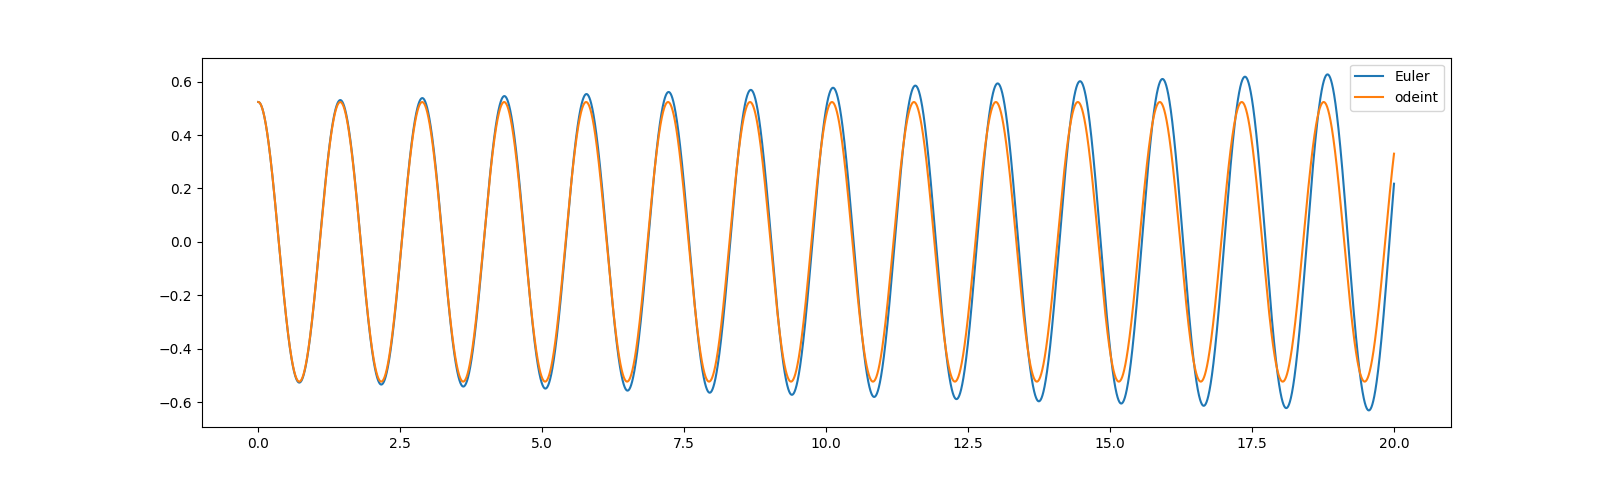
\includegraphics[width=14cm]{Cours/Images/ED2_pendule4.png}
\end{center}
%-------------------------------------------------------------------------------
